\section{Visualizing with \amrvis}
\section{Visualizing with \visit}
\section{Visualizing with \yt}
\yt is a Python package for analyzing and visualizing simulation data.
Originally \yt was written for the {\tt Enzo} code, with focus on
cosmological simulation data.  It has since been refactored to remove
the specific {\tt Enzo}isms, and now can work on various data formats,
such as the BoxLib data from {\tt MAESTRO} and {\tt CASTRO}, HDF5 data
from {\tt FLASH}, and data from the SPH code {\tt Gadget}.  For more
information, see the \yt homepage at {\tt http://yt.enzotools.org/}.

\subsection{Installing \yt}
The easiest way to obtain \yt is through the use of an installation script:
\begin{lstlisting}[language=bash,mathescape=false]
> wget http://hg.enzotools.org/yt/raw-file/stable/doc/install_script.sh
> bash install_script.sh
\end{lstlisting}
By default, this \yt install script will download and install, in its
own isolated environment, all the secondary utilities needed to get \yt
up and running.  Note that this currently includes installing {\it
  hdf5 1.6.9, zlib 1.2.3, bzip2 1.0.5, libpng 1.2.43, freetype 2.4.4,
  Python 2.6.3, numpy 1.5.1, matplotlib 1.0.0, mercurial 1.7.1,
  ipython 0.10, h5py 1.2.0, Cython 0.14, Forthon 0.8.4} as well as a
\yt {\it mercurial} bundle of changes.  You can turn off the automatic
installation of any of these particular packages by setting the
appropriate {\tt INST\_}* variable to zero in the install script;
you may have to then change some of *{\tt \_DIR} variables to point to
your own particular installation of that package.  I usually just let
\yt install its own stuff, which ensures things are working properly.

After the install script has finished, and assuming you let \yt install its own packages, you'll need to {\it prepend} some environment variables with \yt locations so that your system finds those first and stops looking.  For example, the \yt specific information in my {\tt .bashrc} file looks like this
\begin{lstlisting}[language=bash,mathescape=false]
# yt stuff
export YT_DEST=~/install/yt/current/yt-x86_64
export PATH=${YT_DEST}/bin/:$PATH
export PYTHONPATH=${YT_DEST}/lib/python2.6/site-packages/:$PYTHONPATH
export LD_LIBRARY_PATH=${YT_DEST}/lib/:$LD_LIBRARY_PATH
\end{lstlisting}
where I have {\tt ~/install/yt/current} as a soft link to my \yt
installation directory.

\subsection{Working with \yt}
The \yt installation provides both an interactive, {\it iPython}-like,
interface or the ability to import \yt modules for use in a batch
script.  The interactive interface should be in your {\tt \$PATH} if
you've followed the instructions in the previous section; to start it,
simply type {\tt iyt} in a terminal.
\begin{lstlisting}[language=Python]
> iyt

Welcome to yt!


In [1]: 
\end{lstlisting}
Codes like {\tt Enzo} use what are called {\it parameter files} to
describe the general information---number of levels, domain
dimensions, time, etc.---of a a dataset.  \yt likes to grab this
information before working on any specific data; this is accomplished
via the convenience method \textcolor{blue}{\tt load}:
\begin{lstlisting}[language=Python]
In [1]: pf = load(``plt00166'')
\end{lstlisting}
This method returns an instance of the {\tt StaticOutput} class.  One
of the easiest ways of handling plots is via a {\tt PlotCollection}
object
\begin{lstlisting}[language=Python]
In [2]: center = (pf.domain_right_edge + pf.domain_left_edge) / 2.0
In [3]: pc = PlotCollection(pf,center)
\end{lstlisting}
By default, the {\tt PlotCollection} constructor places the center of
the plot to be at the location of peak density.  Here we have
calculated the center of the domain by accessing the lower and upper
domain boundaries via the {\tt numpy} arrays {\tt
  pf.domain\_left\_edge} and {\tt pf.domain\_right\_edge},
respectively.  Note that up until this point, \yt has not actually
loaded the AMR dataset.

Now we would like to take some slices of tfromp in the dataset and
generate some 2-d plots.  To do this, we will use the {\tt
  PlotCollection}'s \textcolor{blue}{\tt add\_slice} method:
\begin{lstlisting}[language=Python]
In [4]: pc.add_slice(``tfromp'',0)
In [5]: pc.add_slice(``tfromp'',1)
In [6]: pc.add_slice(``tfromp'',2)
\end{lstlisting}
The first call to \textcolor{blue}{\tt add\_slice} builds an {\tt
  AMRHierarchy} object associated with {\tt pf}.  The {\tt
  AMRHierarchy} object contains information about the actual dataset,
such as its layout in the simulation domain or on disk.  Building the
hierarchy is expensive, but once it is built the data it contains can
be accessed via attributes and dictionary lookup.  In other words, the
subsequent \textcolor{blue}{\tt add\_slice} operations are relatively
cheap.  The first parameter to the \textcolor{blue}{\tt add\_slice}
method is obviously the variable we want; the second (optional)
parameter specifies an coordinate axis orthogonal to the slice being
made---0 for x, 1 for y, 2 for z.  Now we want to save the plots from
the {\tt PlotCollection}; this is done with the \textcolor{blue}{\tt
  save} method, which takes an optional basename for the generated files:
\begin{lstlisting}[language=Python]
In [7]: pc.save(``my_cool_images'')
\end{lstlisting}
This generates the following image files:
\begin{lstlisting}[language=Python]
Out[7]: 
['my_cool_images_Slice_x_tfromp.png',
 'my_cool_images_Slice_y_tfromp.png',
 'my_cool_images_Slice_z_tfromp.png']
\end{lstlisting}
Figure \ref{fig:yt_slice} shows an example of one of the slice images.
Note that this was a quick and dirty generation of the image---there
is a lot of space around the figure, which can be removed with various
options to the \yt methods.  Also, the user can specify derived
variables, log-scaling, annotations, etc. For more information see the
documentation at {\tt http://yt.enzotools.org/doc/}.

\begin{figure}[!h]\label{fig:yt_slice}
\centering
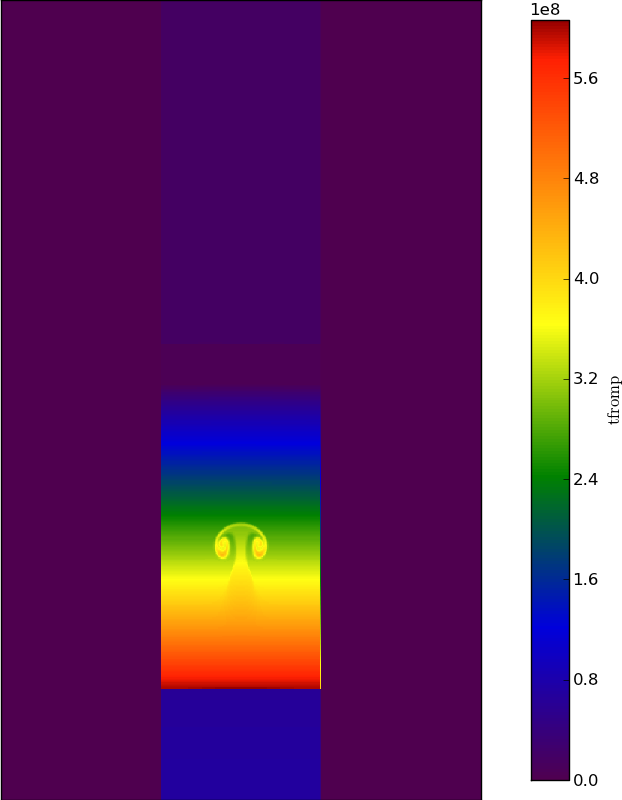
\includegraphics[height=0.4\textheight]{\visfigpath/my_cool_images_Slice_x_tfromp_trim}
\caption{Example slice through 3-d dataset with \yt.}
\end{figure}

When writing a script to use in batch mode, one has to manually import
the import modules needed to work with \yt.  As such, all scripts must
import from the {\tt yt.mods} module, which is essentially a
convenience module that sets up the appropriate \yt namespace.  
%% As an aside, if you want to import a module as another variable in
%% the local namespace---e.g. {\tt import this.module as
%% local\_variable}---then this should be done via the various API's
%% for that particular piece of code.  For example,
For completeness, below is a script containing our example above.
\newpage
\begin{lstlisting}[language=Python]
# load our namespace
from yt.mods import *

# the plotfile I'm interested in
fn = ``plt00166''

# load it into a StaticOutput object
pf = load(fn)

# find the center of the domain
center = (pf.domain_right_edge + pf.domain_left_edge) / 2.0

# associate a PlotCollection with the pf
pc = PlotCollection(pf,center)

# add some slices of tfromp
pc.add_slice(``tfromp'',0)
pc.add_slice(``tfromp'',1)
pc.add_slice(``tfromp'',2)

# save our plots to a files with basename
# ``my_cool_images''
pc.save(``my_cool_images'')
\end{lstlisting}

\subsection{Volume Rendering}
